\begin{pastexam}[label={px:gw3-109-ds-01}]{關務三等資訊處理 109 年 第一題}
（申論；20 分）

資料庫應用中，需要根據主鍵值（Primary Key）建立索引檔，索引檔的建立常使用 B-tree 樹狀結構，今有一串資料，其主鍵值分別為：44, 29, 39, 64, 67, 59, 69, 49，畫出將此串資料建成 order 3 的 B-tree，接著，畫出從此串資料，新增（Insert）主鍵值 55 後 order 3 的 B-tree，最後，畫出從此串資料刪除（Delete）主鍵值 49 後 order 3 的 B-tree。（20 分）
\end{pastexam}

\begin{pastsoln}
\newcommand{\bk}[1]{\begin{tabular}{@{\,}c@{\,}}#1\end{tabular}}
\newcommand{\bkk}[2]{\begin{tabular}{@{\,}c@{\,}|@{\,}c@{\,}}#1 & #2\end{tabular}}
order $3$ 的 B-tree 每個節點最多 $3$ 個子節點、$2$ 個鍵，非根節點至少 $1$ 個鍵，也就是 2-3 樹（資結書第~11.1~節、第~11.2~節）。 插入：放進
該放的葉節點，若變成 $3$ 個鍵，就把中間的鍵往上送、左右分成兩個節點，父節點因此滿了就繼續往上分裂。 刪除照資結書虛擬碼~11.6、11.7：
要刪的鍵在內部節點時，用它的\textbf{後繼}（右子樹最小的鍵）取代，改到葉節點刪；葉節點變空時，先向兄弟借，兄弟只有一個鍵才合併。
題目的「從此串資料新增 55」「從此串資料刪除 49」，本書依序理解：先建好、再插入 55、再從插入 55 後的樹刪除 49；最後也附上直接從原樹刪除
49 的結果。

\textbf{建立}。
\begin{center}
\small
\begin{tabular}{lp{6.4cm}l}
\toprule
插入 & 過程 & 結果（根；第二層） \\
\midrule
44 & 空樹 & $[44]$ \\
29 & 放進根 & $[29, 44]$ \\
39 & $[29, 39, 44]$ 滿了，39 上升成新根 & $[39]$；$[29]$、$[44]$ \\
64 & $> 39$，放進右葉 & $[39]$；$[29]$、$[44, 64]$ \\
67 & 右葉 $[44, 64, 67]$ 分裂，64 上升 & $[39, 64]$；$[29]$、$[44]$、$[67]$ \\
59 & 介於 39、64，放進中葉 & $[39, 64]$；$[29]$、$[44, 59]$、$[67]$ \\
69 & $> 64$，放進右葉 & $[39, 64]$；$[29]$、$[44, 59]$、$[67, 69]$ \\
49 & 中葉 $[44, 49, 59]$ 分裂，49 上升，根變成 $[39, 49, 64]$ 也滿了，再分裂，49 上升成新根 & 見下圖 \\
\bottomrule
\end{tabular}
\end{center}
插入 49 時：中葉分成 $[44]$、$[59]$，49 進根得 $[39, 49, 64]$；根分裂成 $[39]$（子節點 $[29]$、$[44]$）和 $[64]$（子節點 $[59]$、$[67, 69]$），
49 成為新根，樹高增加一層。 建好的 B-tree：
\begin{center}
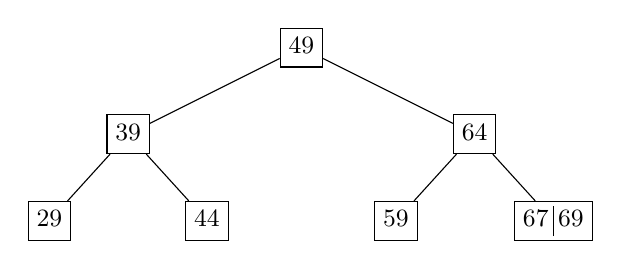
\begin{tikzpicture}[level distance=11mm,level 1/.style={sibling distance=44mm},level 2/.style={sibling distance=20mm},
  every node/.style={draw,inner sep=1.5pt,font=\small}]
\node {\bk{49}}
  child {node {\bk{39}} child {node {\bk{29}}} child {node {\bk{44}}}}
  child {node {\bk{64}} child {node {\bk{59}}} child {node {\bkk{67}{69}}}};
\end{tikzpicture}
\end{center}

\textbf{插入 55}。 $55 > 49$ 往右，$55 < 64$ 往左，到葉 $[59]$，放進去成為 $[55, 59]$，沒有滿，不用分裂：
\begin{center}
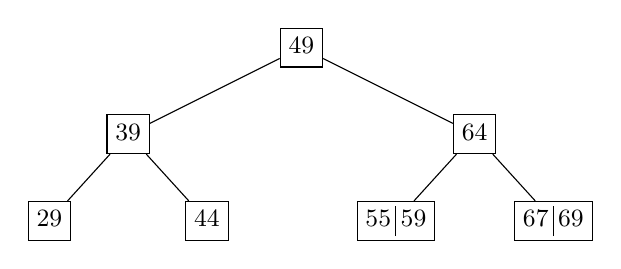
\begin{tikzpicture}[level distance=11mm,level 1/.style={sibling distance=44mm},level 2/.style={sibling distance=20mm},
  every node/.style={draw,inner sep=1.5pt,font=\small}]
\node {\bk{49}}
  child {node {\bk{39}} child {node {\bk{29}}} child {node {\bk{44}}}}
  child {node {\bk{64}} child {node {\bkk{55}{59}}} child {node {\bkk{67}{69}}}};
\end{tikzpicture}
\end{center}

\textbf{刪除 49}（從上圖）。 49 在根（內部節點），後繼是右子樹最小的鍵：從 64 往最左走到葉 $[55, 59]$，後繼是 55。 用 55 取代根的 49，再從葉
$[55, 59]$ 刪掉 55，葉剩 $[59]$，還有 $1$ 個鍵，不會不足，結束：
\begin{center}
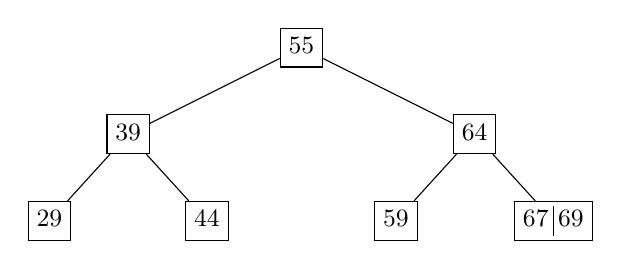
\begin{tikzpicture}[level distance=11mm,level 1/.style={sibling distance=44mm},level 2/.style={sibling distance=20mm},
  every node/.style={draw,inner sep=1.5pt,font=\small}]
\node {\bk{55}}
  child {node {\bk{39}} child {node {\bk{29}}} child {node {\bk{44}}}}
  child {node {\bk{64}} child {node {\bk{59}}} child {node {\bkk{67}{69}}}};
\end{tikzpicture}
\end{center}

\textbf{另一種讀法：直接從原樹（沒有 55）刪除 49}。 後繼是 59，用 59 取代根的 49；葉 $[59]$ 刪掉 59 後變空，不足。 它的右兄弟 $[67, 69]$ 有 $2$ 個鍵，
可以借：父節點的 64 下來到空葉，右兄弟最小的 67 上去取代 64。 結果：
\begin{center}
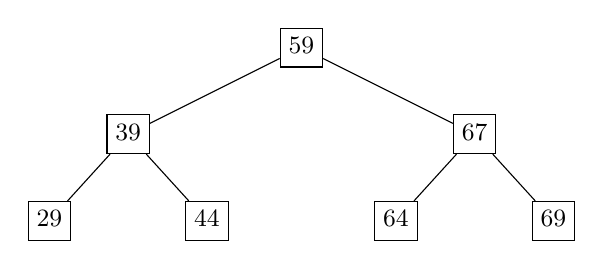
\begin{tikzpicture}[level distance=11mm,level 1/.style={sibling distance=44mm},level 2/.style={sibling distance=20mm},
  every node/.style={draw,inner sep=1.5pt,font=\small}]
\node {\bk{59}}
  child {node {\bk{39}} child {node {\bk{29}}} child {node {\bk{44}}}}
  child {node {\bk{67}} child {node {\bk{64}}} child {node {\bk{69}}}};
\end{tikzpicture}
\end{center}
每一棵都檢查過：所有葉節點在同一層，每個節點 $1$ 或 $2$ 個鍵，中序是遞增的。 刪除內部節點的鍵時用前驅（左子樹最大的鍵）取代也可以，結果
會不同；作答時要寫明用的是哪一種。
\end{pastsoln}
